%% Relatório Técnico – Trabalho Prático AOC II (12029) – UEM
%% Formato baseado nas instruções SBC (sbc_template.pdf): A4, coluna única,
%% margens 3,5/2,5/3,0 cm, Times 12 pt, sem numeração de páginas.
\documentclass[12pt,a4paper]{article}

\usepackage[utf8]{inputenc}
\usepackage[T1]{fontenc}
\usepackage[brazil]{babel}
\usepackage{amsmath}
\usepackage{mathptmx}                 % Times (texto e matemática)
\usepackage[scaled=.92]{helvet}       % Helvetica (legendas)
\usepackage{courier}                  % Courier (e-mails, código)
\usepackage[a4paper,top=3.5cm,bottom=2.5cm,left=3.0cm,right=3.0cm]{geometry}
\usepackage{graphicx}
\usepackage{booktabs}
\usepackage{array}
\usepackage[hyphens]{url}
\Urlmuskip=0mu plus 2mu
\usepackage{listings}
\usepackage{titlesec}
\usepackage{enumitem}
\usepackage{microtype}
\usepackage{xcolor}
\usepackage[font={sf,bf,footnotesize},labelsep=period,skip=6pt,aboveskip=6pt,belowskip=6pt,
            margin=0.8cm,justification=justified,singlelinecheck=on]{caption}

\pagestyle{empty}
\setlength{\parindent}{1.27cm}
\setlength{\parskip}{6pt}
\setlength{\emergencystretch}{2em}
\urlstyle{rm}

% Seções: negrito, 13 pt (subseções 12 pt), à esquerda, 12 pt antes
\titleformat{\section}{\bfseries\fontsize{13}{15}\selectfont}{\thesection.}{0.5em}{}
\titleformat{\subsection}{\bfseries\fontsize{12}{14}\selectfont}{\thesubsection.}{0.5em}{}
\titlespacing*{\section}{0pt}{12pt}{0pt}
\titlespacing*{\subsection}{0pt}{9pt}{0pt}

\renewcommand{\lstlistingname}{Listagem}
\lstset{language=C,captionpos=b,basicstyle=\ttfamily\footnotesize,frame=single,rulecolor=\color{black!40},
        xleftmargin=0.3cm,xrightmargin=0.3cm,aboveskip=4pt,belowskip=2pt,
        breaklines=true,columns=fullflexible,keepspaces=true,showstringspaces=false,
        keywordstyle=\bfseries,commentstyle=\itshape}
\renewcommand{\arraystretch}{1.05}
\newcommand{\tx}{$\times$}
\newcommand{\Tseq}{$T_{seq}$}
\newcommand{\Tpar}{$T_{par}$}

% ------------------------------------------------------------------
% Autores (editar aqui, se necessário)
% ------------------------------------------------------------------
\newcommand{\autores}{Arthur Henrique, Bernardo Wilchen}
\newcommand{\emails}{ra144346@uem.br, ra143177@uem.br}

\begin{document}

\begin{center}
  \vspace*{12pt}
  {\fontsize{16}{19}\selectfont\bfseries Avaliação de Desempenho e Programação Paralela com Threads: Multiplicação de Matrizes, Filtro de Média em Imagens e Contadores Paralelos\par}
  \vspace{12pt}
  {\bfseries\autores\par}
  \vspace{12pt}
  Departamento de Informática (DIN) -- Universidade Estadual de Maringá (UEM)\\
  Maringá -- PR -- Brasil\par
  \vspace{6pt}
  {\fontsize{10}{12}\ttfamily\emails\par}
  \vspace{6pt}
\end{center}

\begin{list}{}{\leftmargin=0.8cm\rightmargin=0.8cm\setlength{\itemsep}{0pt}\setlength{\parsep}{0pt}\setlength{\topsep}{0pt}}
\item[]\noindent\textbf{Resumo.} Este trabalho avalia experimentalmente o efeito do uso de múltiplas threads POSIX (\emph{pthreads}) sobre o desempenho de três aplicações em C: multiplicação de matrizes, filtro de média 3\tx3 em imagens e contadores paralelos. Cada aplicação foi implementada em versão sequencial e paralela (2, 4 e 8 threads) e medida em cinco execuções por configuração, em um Intel Core i7-1165G7 (4 núcleos, 8 threads lógicas). Os resultados são analisados por tempo, \emph{speedup}, eficiência e escalabilidade, e relacionados a multicore, localidade de cache, contenção e coerência de cache (MESI). A multiplicação 1024\tx1024 alcançou \emph{speedup} de 7,16 com 8 threads (acima de 4, o número de núcleos físicos, tratado aqui como anomalia); o contador compartilhado com \emph{mutex} foi até 408 vezes mais lento que o sequencial, enquanto contadores locais chegaram a 2,82.

\vspace{6pt}
\item[]\noindent\textbf{Abstract.} This work experimentally evaluates the effect of POSIX threads on the performance of three C applications: matrix multiplication, a 3\tx3 mean filter on grayscale images, and parallel counters. Each application has a sequential and a parallel version (2, 4 and 8 threads), measured over five runs per configuration on an Intel Core i7-1165G7 (4 cores, 8 logical threads). Results are analyzed in terms of execution time, speedup, efficiency and scalability, and related to multicore execution, cache locality, contention and cache coherence (MESI). The 1024\tx1024 multiplication reached a speedup of 7.16 with 8 threads (above the 4 physical cores, treated as an anomaly); a mutex-protected shared counter was up to 408 times slower than the sequential one, whereas per-thread counters reached 2.82.
\end{list}

\section{Introdução}

Processadores multicore tornaram o paralelismo em nível de thread a principal forma de aumentar o desempenho de aplicações em um único computador. Entretanto, executar um programa com $p$ threads não garante que ele fique $p$ vezes mais rápido: o ganho depende da divisão do trabalho, do custo de criação e sincronização das threads, do uso da hierarquia de memória e do número de núcleos físicos disponíveis [Hennessy and Patterson 2017].

Este relatório documenta o trabalho prático da disciplina Arquitetura e Organização de Computadores II, cujo objetivo é avaliar experimentalmente o impacto de múltiplas threads comparando versões sequenciais e paralelas de três aplicações: (i) multiplicação de matrizes, (ii) filtro de média 3\tx3 sobre imagens em tons de cinza e (iii) contadores paralelos. São analisados o tempo de execução, o \emph{speedup}, a eficiência paralela e a escalabilidade em função do número de threads (2, 4 e 8) e do tamanho da entrada, relacionando os resultados à memória cache e à coerência de cache (protocolo MESI), por meio de análise conceitual.

A Seção~2 descreve as aplicações e as decisões de implementação; a Seção~3, a metodologia e o ambiente experimental; a Seção~4, os resultados; a Seção~5, a análise crítica e a relação com os conceitos arquiteturais; e a Seção~6, as conclusões. Os tempos individuais de todas as execuções e os \emph{prints} de tela estão nos Apêndices~A e~B.

\section{Aplicações e decisões de implementação}

\subsection{Organização do código}

Todas as aplicações foram escritas em C e compiladas com \texttt{gcc}. A multiplicação de matrizes (\texttt{mult\_mat.c}) e o filtro de imagens (\texttt{imagens.c}) compartilham o arquivo \texttt{linhas.h}, que contém a estrutura de trabalho de cada thread, a divisão em faixas de linhas, a criação/junção das threads e a medição de tempo; assim, ambas usam exatamente a mesma estratégia de paralelização e o mesmo método de medição. Os contadores (\texttt{contadores.c}) formam um programa independente, pois seu paralelismo não é baseado em divisão de linhas.

Cada programa recebe, na linha de comando, o modo de execução e a quantidade de threads: \texttt{./mult\_mat S 1024} (sequencial), \texttt{./mult\_mat P 1024 4} (paralelo com 4 threads), \texttt{./contadores A 8} (contador compartilhado com 8 threads), e assim por diante. A quantidade de threads é restrita a 2, 4 ou 8, como especificado.

\subsection{Divisão do trabalho nas aplicações baseadas em linhas}

Nas versões paralelas, as $n$ linhas da saída são divididas em $p$ faixas contíguas; a thread $i$ processa as linhas de $\lfloor i\,n/p \rfloor$ até $\lfloor (i+1)\,n/p \rfloor - 1$. Como $n$ é potência de 2 e $p\in\{2,4,8\}$, as faixas têm o mesmo tamanho, de modo que não há cálculo redundante nem desbalanceamento de carga: cada linha de saída é calculada por exatamente uma thread. A Listagem~\ref{lst:div} mostra o trecho central, que também delimita a região medida.

\begin{lstlisting}[float=tp,caption={Criação, distribuição e junção das threads em \texttt{linhas.h}, com a região cronometrada.},label={lst:div}]
clock_gettime(CLOCK_MONOTONIC, &t0);
for (int i = 0; i < p; i++) {            /* distribuicao */
    partes[i] = dados;
    partes[i].inicio = i * dados.n / p;
    partes[i].fim    = (i + 1) * dados.n / p;
    checar(pthread_create(&threads[i], NULL, calcular, &partes[i]));
}
for (int i = 0; i < p; i++)              /* espera */
    checar(pthread_join(threads[i], NULL));
clock_gettime(CLOCK_MONOTONIC, &t1);
\end{lstlisting}

\textbf{Sincronização.} Nessas duas aplicações os dados compartilhados são apenas lidos (matrizes $A$ e $B$; imagem de entrada), e cada thread escreve somente em sua própria faixa da saída. Não há, portanto, condição de corrida, e o único mecanismo de sincronização necessário é \texttt{pthread\_join}, que garante que todas as faixas estejam concluídas antes de a saída ser lida ou comparada.

\subsection{Multiplicação de matrizes}

A versão sequencial calcula $C = A \times B$ com três laços (\texttt{i}, \texttt{j}, \texttt{k}), com $A$ e $B$ em ordem de linha (\emph{row-major}) e um acumulador local \texttt{soma} por elemento de $C$ (Listagem~\ref{lst:mm}). As matrizes $A$ e $B$ são de \texttt{int} e $C$ de \texttt{long}. Foram usados os arquivos \texttt{A\_n.txt} e \texttt{B\_n.txt}, gerados pelo código fornecido na especificação (\texttt{srand(12345)}), para $n \in \{256, 512, 1024\}$. A leitura dos arquivos é feita antes do cronômetro e não entra nas medições. A versão paralela chama a mesma função \texttt{mult\_seq} sobre a faixa de linhas de cada thread, de modo que sequencial e paralela executam exatamente o mesmo código de cálculo.

\begin{lstlisting}[float=tp,caption={Núcleo de \texttt{mult\_seq}, usado nas versões sequencial (\texttt{inicio}=0, \texttt{fim}=$n$) e paralela.},label={lst:mm}]
for (int i = inicio; i < fim; i++)
  for (int j = 0; j < n; j++) {
    long soma = 0;
    for (int k = 0; k < n; k++)
      soma += (long) A[i*n + k] * B[k*n + j];
    C[i*n + j] = soma;
  }
\end{lstlisting}

\subsection{Filtro de média 3\tx3}

Cada pixel interno da saída recebe a média inteira (soma dos 9 vizinhos dividida por 9, com truncamento) da vizinhança 3\tx3 da imagem de entrada; os pixels das bordas são copiados sem alteração. A saída é gravada em um \emph{buffer} separado, e não sobre a entrada, o que elimina dependências entre linhas e permite que as threads leiam as linhas vizinhas à sua faixa (linhas de fronteira) sem conflito.

Os arquivos PNG fornecidos (256\tx256, 512\tx512 e 1024\tx1024, escala de cinza) são sintéticos: um gradiente horizontal, anéis concêntricos e um padrão suave, respectivamente. Para evitar o uso de biblioteca de decodificação PNG no programa em C, o \emph{script} \texttt{preparar.py} (Pillow) converte cada PNG em um arquivo \texttt{.raw} de 8 bits por pixel, que o programa lê antes do cronômetro. O custo do filtro não depende do conteúdo da imagem, apenas de suas dimensões.

\subsection{Contadores paralelos}

O contador deve ir de 0 a $10^8$. São quatro variantes: \textbf{sequencial} (um laço de $10^8$ incrementos), \textbf{versão A} (todas as threads incrementam a mesma variável global \texttt{cont\_global}, e cada incremento é protegido por \texttt{pthread\_mutex\_lock/unlock}) e \textbf{versão B} (cada thread incrementa um contador local sobre seu intervalo de $10^8/p$ incrementos, e os parciais são somados após o \texttt{pthread\_join}). A Listagem~\ref{lst:cont} mostra as duas funções de thread.

\begin{lstlisting}[float=tp,caption={Funções executadas pelas threads nas versões A e B dos contadores.},label={lst:cont}]
void *thread_A(void *arg) {            /* contador compartilhado */
    Args *a = (Args *) arg;
    for (long i = a->inicio; i < a->fim; i++) {
        pthread_mutex_lock(&mutex_global);
        cont_global++;
        pthread_mutex_unlock(&mutex_global);
    }
    return NULL;
}
void *thread_B(void *arg) {            /* contador local */
    volatile long local = 0;
    Args *a = (Args *) arg;
    for (long i = a->inicio; i < a->fim; i++) local++;
    a->parcial = local;                /* unica escrita compartilhada */
    return NULL;
}
\end{lstlisting}

As variáveis do contador sequencial e do contador local (versão B) são declaradas \texttt{volatile} para impedir que o compilador, com \texttt{-O2}, elimine o laço ou o substitua pela atribuição direta do resultado final. Assim, as versões sequencial e B realizam o mesmo trabalho por incremento (um acesso à memória), e a comparação entre elas é justa. Vale notar que \texttt{volatile} não garante atomicidade: na versão A, a correção vem exclusivamente do \emph{mutex}. Na versão B, o único dado escrito por uma thread e lido depois por outra é o campo \texttt{parcial}, escrito uma única vez ao final.

\subsection{Verificação de corretude}

\textbf{Matrizes e imagens.} O programa aceita a variável de ambiente \texttt{SAIDA}, que grava a saída completa (matriz $C$ ou imagem filtrada) em um arquivo binário. Para cada aplicação e cada tamanho, a saída sequencial foi comparada byte a byte, com \texttt{cmp}, com as saídas paralelas de 2, 4 e 8 threads (18 comparações, Figura~\ref{fig:s4} do Apêndice~B); todas resultaram em arquivos idênticos. Os programas também imprimem valores de controle (\texttt{C[0][0]} e \texttt{C[n-1][n-1]}; pixel central), usados na inspeção visual. \textbf{Contadores.} O \emph{script} de coleta confere, em toda execução, que a saída contém \texttt{Contador: 100000000} e aborta caso contrário; as 155 execuções foram registradas, portanto todas passaram na verificação.

\section{Metodologia experimental}

\subsection{Ambiente experimental}

A Tabela~\ref{tab:amb} resume o ambiente. Todos os experimentos foram executados no mesmo computador, em 22/11/2026.

\begin{table}[!htbp]
\caption{Ambiente experimental.}
\label{tab:amb}
\centering\small
\begin{tabular}{@{}p{3.6cm}p{10.2cm}@{}}
\toprule
Computador & Dell Inspiron 3501 (notebook) \\
Processador & Intel Core i7-1165G7 (11ª geração), 2,80 GHz nominal \\
Núcleos / threads lógicas & 4 núcleos físicos, 2 threads por núcleo (Hyper-Threading), 8 CPUs lógicas, 1 soquete \\
Frequência & Dinâmica; até 4,7 GHz em \emph{turbo} [Intel 2020]; \texttt{lscpu} indicou escalonamento de frequência ativo \\
Cache & L3 de 12 MB compartilhada [Intel 2020]; L2 de 1,25 MiB e L1 de dados de 48 KiB por núcleo (especificação pública do modelo); linhas de 64 bytes \\
Memória RAM & 16 GB nominais (15 GiB reportados por \texttt{free -h}); \emph{swap} de 2 GiB (sem uso durante a captura) \\
Sistema operacional & Linux Mint 22.3 (\emph{Zena}), base Ubuntu 24.04 (\emph{noble}), \emph{kernel} 6.8.0-147-generic, Cinnamon 6.6.9 / X11 \\
Compilador & \texttt{gcc} (Ubuntu 13.3.0-6ubuntu2$\sim$24.04.1) 13.3.0 \\
Opções de compilação & \texttt{-O2 -Wall -Wextra -pthread} \\
Biblioteca de threads & POSIX Threads (\emph{pthreads}) \\
\bottomrule
\end{tabular}
\end{table}

% CONFIRMAR/COMPLEMENTAR: programas abertos durante os testes e modo de energia (bateria/tomada).
\textbf{Condições de execução e limitações.} Os testes foram executados em um terminal dentro de uma sessão gráfica (Cinnamon/X11). Não foram aplicados isolamento de núcleos (\texttt{isolcpus}, \texttt{taskset}), fixação do \emph{governor} de frequência nem desativação do Hyper-Threading; assim, processos do sistema e da sessão gráfica podem ter competido pelos núcleos, e a frequência do processador, que em um notebook varia com limites térmicos e de potência, não foi controlada. Não foram usados contadores de hardware (por exemplo, \texttt{perf}), o que limita as conclusões sobre cache e coerência a interpretações teóricas (Seção~5). O processador possui apenas 4 núcleos físicos: as configurações com 8 threads usam as 8 CPUs lógicas, que compartilham as unidades de execução e as caches L1/L2 de cada núcleo.

\subsection{Medição do tempo}

O tempo foi medido com \texttt{clock\_gettime(CLOCK\_MONOTONIC)}, que fornece resolução de nanossegundos e não é afetado por ajustes do relógio do sistema; a diferença entre as duas leituras é convertida para segundos (\texttt{double}) e, neste relatório, apresentada \textbf{em milissegundos (ms) em todas as tabelas e gráficos}. O mesmo método é usado em todas as versões. Nas versões paralelas, o intervalo cronometrado inclui a criação das threads, a distribuição do trabalho, a sincronização (\emph{mutex}, na versão A) e a espera por \texttt{pthread\_join}; na versão B dos contadores, inclui também a soma final dos parciais. Não são incluídos a compilação, a geração das matrizes e a leitura dos arquivos de entrada (matrizes e imagens), realizadas antes do primeiro \texttt{clock\_gettime}.

\subsection{Procedimento e estatísticas}

O \emph{script} \texttt{coleta.sh} executa, para cada uma de 5 repetições, todas as configurações: multiplicação e filtro com $n\in\{256,512,1024\}$ e modos S, P2, P4 e P8, e contadores nos modos S, A2, A4, A8, B2, B4 e B8 (31 configurações; 155 execuções). As repetições são intercaladas, isto é, cada rodada percorre todas as configurações, o que distribui eventuais variações do estado da máquina (temperatura, frequência, tarefas em segundo plano) entre as configurações em vez de concentrá-las em uma só. Cada execução é um novo processo, com as mesmas entradas, e seu tempo é registrado em \texttt{tempos.csv}.

Como medida representativa foi adotada a \textbf{mediana} dos 5 tempos, por ser robusta a valores atípicos, que ocorreram (por exemplo, na multiplicação sequencial 512\tx512, o tempo máximo é 63\% acima da mediana). Como medidas de dispersão são informados o \textbf{mínimo}, o \textbf{máximo} e o \textbf{desvio-padrão amostral} ($\sigma$, com divisor $n-1$). Os tempos individuais estão no Apêndice~A.

\subsection{Métricas}

Com \Tseq{} e \Tpar{} dados pelas medianas, o \emph{speedup} e a eficiência para $p$ threads são
\begin{equation*}
S = \frac{T_{seq}}{T_{par}}, \qquad E = \frac{S}{p}\quad(\text{também em \%}),
\end{equation*}
onde \Tseq{} é a mediana da versão sequencial da mesma aplicação e do mesmo tamanho de entrada. Para os contadores, \Tseq{} é o contador sequencial. Valores de $S>1$ indicam aceleração; $S=1$, desempenho equivalente; $S<1$, versão paralela mais lenta. Exemplo de cálculo (multiplicação 512\tx512, $p=4$): $S = 289{,}05/68{,}52 = 4{,}22$ e $E = 4{,}22/4 = 1{,}05 = 105\%$.

\section{Resultados}

Nas tabelas a seguir, os tempos estão em ms; \emph{Seq.} indica a versão sequencial ($p=1$). Os valores de $S$ e $E$ foram calculados a partir das medianas, sem arredondamento intermediário.

\subsection{Multiplicação de matrizes}

\begin{table}[!htbp]
\caption{Multiplicação de matrizes: tempos (ms), \emph{speedup} e eficiência (5 execuções).}
\label{tab:mult}
\centering\small
\begin{tabular}{@{}rrrrrrrr@{}}
\toprule
$n$ & $p$ & Mediana & Mín. & Máx. & $\sigma$ & $S$ & $E$ (\%) \\
\midrule
256 & Seq. & 27,3 & 25,3 & 31,7 & 2,95 & 1,00 & 100 \\
256 & 2 & 15,5 & 13,2 & 22,2 & 3,50 & 1,76 & 87,9 \\
256 & 4 & 10,1 & 7,31 & 14,4 & 3,41 & 2,71 & 67,8 \\
256 & 8 & 11,0 & 7,02 & 12,2 & 2,00 & 2,47 & 30,9 \\
\midrule
512 & Seq. & 289 & 277 & 470 & 81,0 & 1,00 & 100 \\
512 & 2 & 145 & 126 & 174 & 18,7 & 2,00 & 99,8 \\
512 & 4 & 68,5 & 65,8 & 135 & 30,0 & 4,22 & 105,5 \\
512 & 8 & 67,2 & 54,9 & 78,4 & 8,52 & 4,30 & 53,8 \\
\midrule
1024 & Seq. & 6261 & 5893 & 6682 & 305 & 1,00 & 100 \\
1024 & 2 & 1925 & 1707 & 2206 & 178 & 3,25 & 162,6 \\
1024 & 4 & 882 & 788 & 930 & 63,7 & 7,10 & 177,5 \\
1024 & 8 & 875 & 780 & 886 & 48,2 & 7,16 & 89,5 \\
\bottomrule
\end{tabular}
\end{table}

\begin{figure}[!htbp]
\centering
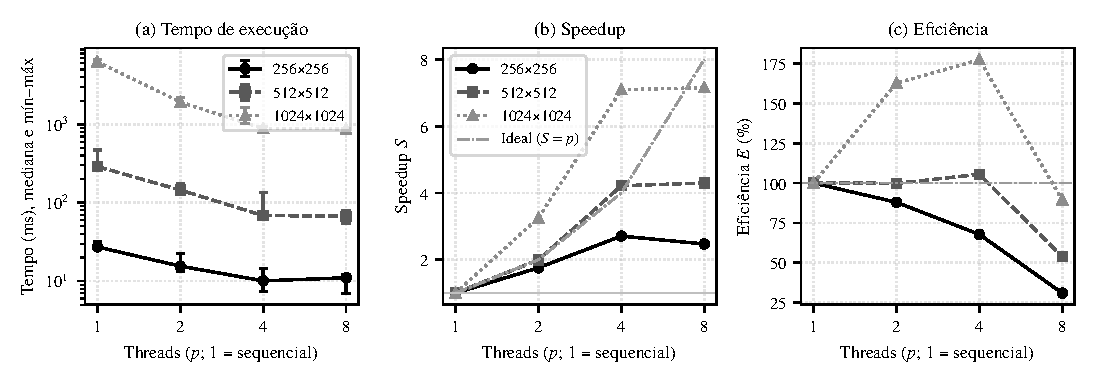
\includegraphics[width=\textwidth]{fig/fig_mult.pdf}
\caption{Multiplicação de matrizes: (a) tempo (mediana e intervalo mín--máx, eixo logarítmico), (b) \emph{speedup} e (c) eficiência, em função do número de threads ($p=1$ é a versão sequencial).}
\label{fig:mult}
\end{figure}

A Tabela~\ref{tab:mult} e a Figura~\ref{fig:mult} mostram que o desempenho melhora com $p$ até 4 threads em todos os tamanhos, e que passar de 4 para 8 threads praticamente não traz ganho: em $n=1024$ o tempo cai de 882 ms para 875 ms (0,8\%) e em $n=512$ de 68,5 ms para 67,2 ms (2\%), diferenças menores que a dispersão observada; em $n=256$ a versão com 8 threads é até mais lenta (11,0 ms contra 10,1 ms). O \emph{speedup} cresce com o tamanho da entrada: com 4 threads, é 2,71 ($n=256$), 4,22 ($n=512$) e 7,10 ($n=1024$).

Dois pontos merecem atenção. Primeiro, para $n=1024$ a eficiência chega a 163\% ($p=2$) e 177\% ($p=4$), isto é, o \emph{speedup} medido supera o número de threads, o que é teoricamente incomum e é discutido na Seção~5.2. Segundo, a dispersão é grande nas execuções curtas (coeficiente de variação de até 37\%, em $n=512$, $p=4$); em $n=1024$ ela é menor (5\% a 9\%).

\subsection{Filtro de média em imagens}

\begin{table}[!htbp]
\caption{Filtro de média 3\tx3: tempos (ms), \emph{speedup} e eficiência (5 execuções).}
\label{tab:img}
\centering\small
\begin{tabular}{@{}rrrrrrrr@{}}
\toprule
Resolução & $p$ & Mediana & Mín. & Máx. & $\sigma$ & $S$ & $E$ (\%) \\
\midrule
256 & Seq. & 0,459 & 0,448 & 0,597 & 0,072 & 1,00 & 100 \\
256 & 2 & 0,418 & 0,373 & 0,510 & 0,054 & 1,10 & 54,9 \\
256 & 4 & 0,452 & 0,369 & 0,713 & 0,136 & 1,01 & 25,4 \\
256 & 8 & 0,491 & 0,407 & 0,527 & 0,046 & 0,93 & 11,7 \\
\midrule
512 & Seq. & 2,63 & 1,96 & 3,62 & 0,654 & 1,00 & 100 \\
512 & 2 & 1,38 & 1,13 & 1,70 & 0,227 & 1,90 & 94,9 \\
512 & 4 & 1,21 & 0,765 & 1,98 & 0,486 & 2,17 & 54,3 \\
512 & 8 & 1,15 & 0,860 & 1,25 & 0,189 & 2,28 & 28,5 \\
\midrule
1024 & Seq. & 9,35 & 8,52 & 11,1 & 1,05 & 1,00 & 100 \\
1024 & 2 & 5,78 & 4,47 & 9,25 & 1,87 & 1,62 & 80,9 \\
1024 & 4 & 3,86 & 2,27 & 4,52 & 0,884 & 2,42 & 60,6 \\
1024 & 8 & 4,40 & 3,45 & 4,96 & 0,603 & 2,13 & 26,6 \\
\bottomrule
\end{tabular}
\end{table}

\begin{figure}[!htbp]
\centering
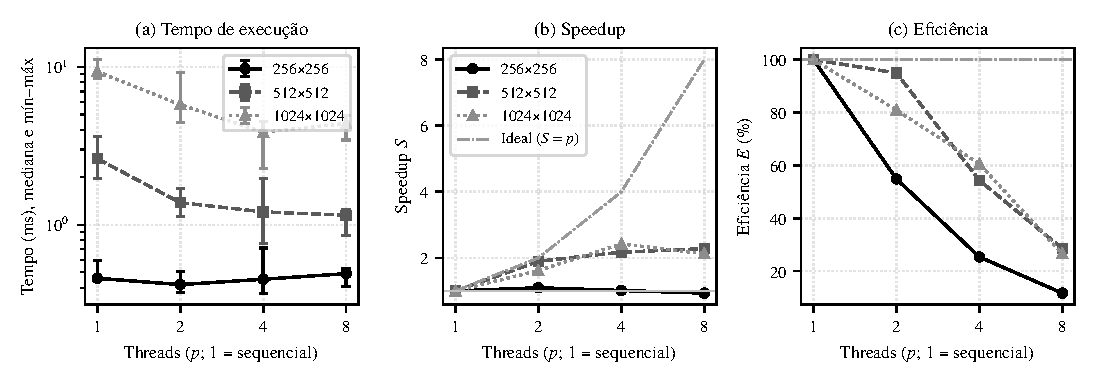
\includegraphics[width=\textwidth]{fig/fig_img.pdf}
\caption{Filtro de média 3\tx3: (a) tempo (mediana e intervalo mín--máx), (b) \emph{speedup} e (c) eficiência.}
\label{fig:img}
\end{figure}

Os ganhos do filtro são bem mais modestos (Tabela~\ref{tab:img} e Figura~\ref{fig:img}). Para 256\tx256 não há aceleração: o tempo sequencial é de apenas 0,46 ms e o \emph{speedup} fica entre 0,93 e 1,10. Para 512\tx512 e 1024\tx1024 há aceleração, mas o melhor resultado é 2,42 (1024\tx1024, $p=4$), e com 8 threads o desempenho piora em relação a 4 threads em 1024\tx1024 ($S=2{,}13$ contra 2,42). A eficiência cai de 55--95\% com 2 threads para 12--29\% com 8 threads. Também aqui a dispersão é alta (coeficiente de variação de 10\% a 40\%), pois os tempos são de apenas alguns milissegundos.

\subsection{Contadores paralelos}

\begin{table}[!htbp]
\caption{Contadores ($10^8$ incrementos): tempos (ms), \emph{speedup} e eficiência (5 execuções). A: contador compartilhado com \emph{mutex}; B: contadores locais.}
\label{tab:cont}
\centering\small
\begin{tabular}{@{}llrrrrrr@{}}
\toprule
Versão & $p$ & Mediana & Mín. & Máx. & $\sigma$ & $S$ & $E$ (\%) \\
\midrule
Seq. & 1 & 80,2 & 75,1 & 108 & 13,0 & 1,00 & 100 \\
\midrule
A & 2 & 17870 & 15943 & 21099 & 2049 & 0,0045 & 0,225 \\
A & 4 & 23382 & 19131 & 25414 & 2424 & 0,0034 & 0,086 \\
A & 8 & 32733 & 25602 & 38467 & 5375 & 0,0025 & 0,031 \\
\midrule
B & 2 & 47,4 & 43,7 & 56,2 & 4,92 & 1,69 & 84,6 \\
B & 4 & 28,4 & 27,7 & 31,9 & 1,90 & 2,82 & 70,6 \\
B & 8 & 73,6 & 66,6 & 92,0 & 9,91 & 1,09 & 13,6 \\
\bottomrule
\end{tabular}
\end{table}

\begin{figure}[!htbp]
\centering
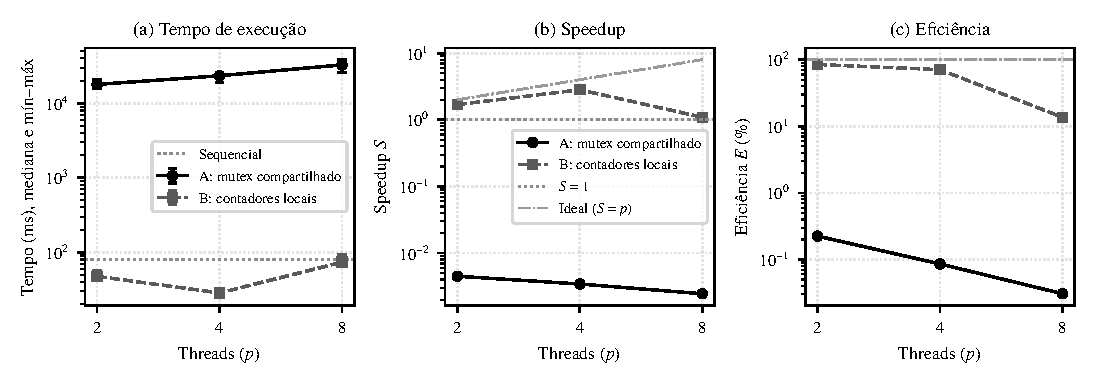
\includegraphics[width=\textwidth]{fig/fig_cont.pdf}
\caption{Contadores: (a) tempo (mediana e intervalo mín--máx), (b) \emph{speedup} e (c) eficiência; eixos verticais em escala logarítmica.}
\label{fig:cont}
\end{figure}

A diferença entre as versões é de ordens de grandeza (Tabela~\ref{tab:cont} e Figura~\ref{fig:cont}). Com o contador compartilhado protegido por \emph{mutex} (A), o tempo é de 17,9 s com 2 threads, 23,4 s com 4 e 32,7 s com 8, contra 80,2 ms do contador sequencial: a versão paralela é, respectivamente, 223, 291 e 408 vezes \textbf{mais lenta} que a sequencial ($S$ entre 0,0045 e 0,0025), e o tempo \emph{aumenta} com o número de threads. Com contadores locais (B), o tempo é 47,4 ms ($p=2$), 28,4 ms ($p=4$) e 73,6 ms ($p=8$), com $S$ de 1,69, 2,82 e 1,09. Em relação à versão A, a versão B é 377, 823 e 445 vezes mais rápida com 2, 4 e 8 threads, respectivamente. Dividindo o tempo da versão A por $10^8$, o custo médio por incremento é de 179 ns, 234 ns e 327 ns (2, 4 e 8 threads), contra 0,8 ns no sequencial.

\subsection{Escalabilidade}

A Figura~\ref{fig:comp} compara o \emph{speedup} das três aplicações na maior entrada, e a Figura~\ref{fig:nsmac} mostra o custo por operação da multiplicação sequencial, usado na análise da Seção~5.2.

\begin{figure}[!htbp]
\centering
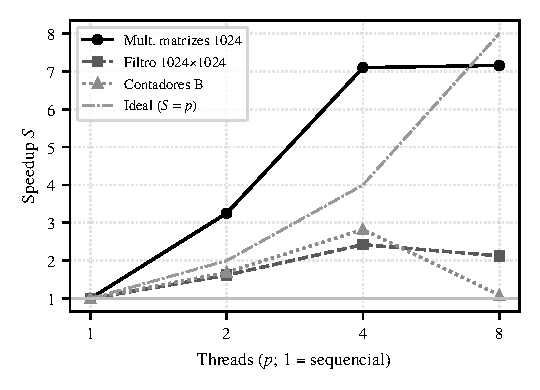
\includegraphics[width=0.62\textwidth]{fig/fig_comp.pdf}
\caption{\emph{Speedup} na maior entrada: multiplicação 1024\tx1024, filtro 1024\tx1024 e contadores (versão B).}
\label{fig:comp}
\end{figure}

\begin{figure}[!htbp]
\centering
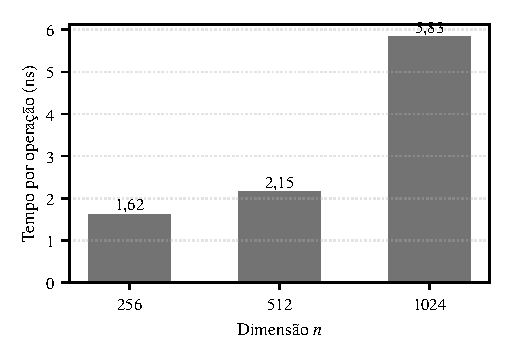
\includegraphics[width=0.58\textwidth]{fig/fig_nsmac.pdf}
\caption{Multiplicação sequencial: tempo mediano por operação de multiplicação-acumulação ($T_{seq}/n^3$).}
\label{fig:nsmac}
\end{figure}

\textbf{Em relação ao tamanho da entrada.} O custo da multiplicação sequencial não cresce como o esperado $O(n^3)$ (fator 8 a cada dobro de $n$): o tempo foi multiplicado por 10,6 de 256 para 512 e por 21,7 de 512 para 1024, e o tempo por operação passou de 1,62 ns para 2,15 ns e 5,83 ns (Figura~\ref{fig:nsmac}). No filtro, o tempo sequencial cresceu 5,7 vezes e 3,6 vezes (o número de pixels cresce 4 vezes a cada passo). Em ambas as aplicações o \emph{speedup} aumenta com o tamanho da entrada, porque o custo fixo de criar e juntar as threads é diluído por mais trabalho útil.

\textbf{Em relação ao número de threads.} A melhor configuração variou: 4 threads na multiplicação 256\tx256, no filtro 1024\tx1024 e nos contadores B; 2 threads no filtro 256\tx256; e empate técnico entre 4 e 8 threads na multiplicação 512\tx512 e 1024\tx1024 e no filtro 512\tx512 (diferenças de 1\% a 5\%, dentro da dispersão). Em nenhum caso usar 8 threads foi claramente melhor que 4, e em vários foi pior (multiplicação 256, filtro 256 e 1024, contadores B).

\section{Análise crítica e relação com os conceitos da disciplina}

Nesta seção, os fatos \textbf{medidos} (tempos, \emph{speedups}) são distinguidos das \textbf{interpretações} teóricas, que não foram verificadas com contadores de hardware e devem ser lidas como hipóteses coerentes com os dados.

\subsection{Multicore, Hyper-Threading e número de threads}

O processador tem 4 núcleos físicos e 8 CPUs lógicas. Medido: o ganho máximo ocorre com até 4 threads e a passagem de 4 para 8 threads não traz ganho claro (Seção~4.4). Interpretação: as duas threads lógicas de um núcleo compartilham unidades de execução, caches L1/L2 e largura de banda, de modo que 8 threads não equivalem a 8 núcleos; o ganho adicional do \emph{multithreading} simultâneo depende de haver ociosidade a ser preenchida e, em cargas que já mantêm o núcleo ocupado, é pequeno. Além disso, mais threads significam mais custo de criação, escalonamento e junção, e, em um notebook, possivelmente menor frequência com todos os núcleos ativos (limite de potência/temperatura, não medido). Na versão B dos contadores, o tempo com 8 threads (73,6 ms) é 2,6 vezes o tempo com 4 threads (28,4 ms), um efeito maior que o esperado apenas pelo compartilhamento do núcleo; não foi possível, com os dados coletados, determinar sua causa.

\subsection{Cache, localidade e a multiplicação de matrizes}

Na multiplicação, cada elemento $C_{ij}$ percorre a linha $i$ de $A$ (acesso sequencial, boa localidade espacial) e a coluna $j$ de $B$ (acesso com passo de $4n$ bytes, ruim localidade espacial). Para $n=1024$, o passo é de 4096 bytes, uma página e uma potência de 2, o que tende a mapear os elementos de uma coluna em poucos conjuntos da cache, e a matriz $B$ (4 MiB) excede a L2 de um núcleo (1,25 MiB), embora caiba na L3 (12 MB). Medido: o custo por operação da versão sequencial sobe de 1,62 ns ($n=256$) para 5,83 ns ($n=1024$), um aumento de 3,6 vezes (Figura~\ref{fig:nsmac}). Interpretação: a perda de localidade (mais acessos servidos pela L3 em vez de L2/L1) é a explicação mais plausível para esse aumento; ela é consistente com a teoria [Hennessy and Patterson 2017, Drepper 2007], mas não foi confirmada por contadores de falhas de cache.

\textbf{Eficiência acima de 100\%.} Para $n=1024$, o tempo por operação ``por núcleo'' ($T_{par}\cdot p/n^3$) é 3,59 ns ($p=2$) e 3,29 ns ($p=4$), contra 5,83 ns da versão sequencial, isto é, cada thread paralela executou suas operações mais rápido que a thread sequencial. Como as duas versões executam o mesmo código de cálculo, o resultado é um fato medido (5 repetições consistentes; mínimo sequencial 5,89 s contra máximo de 4 threads de 0,93 s), mas sua causa \emph{não foi isolada}. Hipóteses: (i) o comportamento da hierarquia de memória (conflitos de cache, TLB, pré-busca e L3 compartilhada) diante do padrão de acesso por coluna pode diferir quando vários núcleos executam concorrentemente; (ii) o estado de frequência/potência do notebook pode variar entre uma execução sequencial longa (cerca de 6 s) e execuções paralelas mais curtas; (iii) a linha de base sequencial é particularmente desfavorável por usar o laço ingênuo \texttt{ijk}; uma ordem de laços mais amigável à cache (\texttt{ikj}) ou blocagem reduziria bastante \Tseq{} e, com isso, os \emph{speedups}. Esses valores devem ser lidos como razão medida em relação a essa linha de base, e não como evidência de ganho ``acima do ideal''. Uma validação futura exigiria \texttt{perf stat} (faltas de L1/L2/LLC), \emph{governor} fixo em \texttt{performance} e fixação de threads com \texttt{taskset}.

\subsection{Filtro de imagens: pouco trabalho por byte e sobrecarga}

O filtro faz 9 leituras de 1 byte e poucas operações aritméticas por pixel, ou seja, tem baixa intensidade aritmética e é sensível à memória. Medido: com 4 threads a eficiência é de apenas 25\% a 61\%, e em 256\tx256 não há ganho. Interpretação: com tempos sequenciais de 0,46 ms, 2,6 ms e 9,3 ms, a criação e junção de threads (tipicamente dezenas de microssegundos por thread, ordem de grandeza não medida neste trabalho), a dispersão do escalonador e a banda de memória compartilhada pesam muito mais do que na multiplicação, cujo trabalho por thread é bem maior. É o comportamento previsto pela lei de Amdahl: a parcela que não escala (criação/junção, acesso à memória) limita o ganho [Amdahl 1967]. O aumento do \emph{speedup} com a resolução (Seção~4.4) é compatível com a diluição desse custo fixo.

\subsection{Contadores: mutex compartilhado versus contadores locais}

\textbf{Medido:} o contador A é mais lento que o sequencial (223 a 408 vezes) e piora com mais threads; o contador B escala até 4 threads ($S=2{,}82$). Em A, as threads trabalham em série na seção crítica: apenas uma incrementa por vez, de modo que não há paralelismo útil, e a cada incremento se pagam a aquisição e a liberação do \emph{mutex} (operações atômicas) e a disputa por ele (contenção). Em B, as threads não se comunicam durante o laço e só a soma final de $p$ valores é serial; esta é a razão do bom desempenho. A diferença de custo por incremento (0,3--0,8 ns em B e no sequencial contra 179--327 ns em A) mostra que o custo da sincronização por incremento supera em muito o custo do trabalho que ela protege (um incremento).

\textbf{Interpretação sobre as causas do custo de A.} Duas fontes são plausíveis e não foram medidas separadamente: (a) a movimentação, entre os caches dos núcleos, das linhas que contêm a trava e \texttt{cont\_global} (coerência de cache, Seção~5.5); e (b) o caminho lento do \emph{mutex} sob contenção, em que threads bloqueiam no \emph{kernel} (\emph{futex}) e são reescalonadas, o que envolve chamadas de sistema e trocas de contexto. Uma inspeção dos símbolos do binário (\texttt{nm}) mostra \texttt{mutex\_global} em \texttt{0x4060} (40 bytes) e \texttt{cont\_global} em \texttt{0x4088}: o campo de trava e o contador ficam em linhas de 64 bytes distintas, de modo que, ao alternar de núcleo, até duas linhas precisam migrar a cada incremento. O crescimento do custo com $p$ (179, 234 e 327 ns) é coerente com mais disputantes e mais trocas de posse, mas também isso é interpretação. Em termos de projeto, a lição é reduzir ao mínimo o estado compartilhado e escrito com frequência: usar acumuladores locais e combinar os resultados ao final (como em B), em vez de sincronizar a cada operação.

\subsection{Coerência de cache e protocolo MESI (análise conceitual)}

Em um multicore com caches privadas, a coerência garante que todos os núcleos vejam um valor consistente de cada linha de cache. No protocolo MESI [Papamarcos and Patel 1984], cada linha em uma cache privada está em um de quatro estados: \textbf{M} (\emph{Modified}: única cópia válida, alterada em relação à memória), \textbf{E} (\emph{Exclusive}: única cópia, igual à memória), \textbf{S} (\emph{Shared}: possivelmente várias cópias, todas iguais à memória) e \textbf{I} (\emph{Invalid}). Ler uma linha que outro núcleo mantém em M obriga a transferi-la (com atualização da memória) e leva as duas cópias a S; escrever em uma linha em S ou I exige obter a posse exclusiva, invalidando as demais cópias (\emph{read for ownership}), que passam a I. Processadores Intel usam variantes desse protocolo (por exemplo, com o estado adicional \emph{Forward}), o que não altera a discussão qualitativa abaixo. A Tabela~\ref{tab:mesi} relaciona cada aplicação ao comportamento esperado e ao que foi efetivamente medido.

\begin{table}[!htbp]
\caption{Coerência de cache: interpretação teórica (MESI) \emph{versus} o que foi medido. Nenhum evento de coerência foi medido diretamente.}
\label{tab:mesi}
\centering\footnotesize
\begin{tabular}{@{}p{2.5cm}p{5.8cm}p{5.5cm}@{}}
\toprule
Aplicação & Interpretação teórica (não medida) & Evidência medida \\
\midrule
Multiplicação & $A$ e $B$ só são lidas: linhas em S nos vários núcleos, sem invalidações. Cada thread escreve em sua faixa de $C$ (linhas em M/E privadas); no máximo uma linha na fronteira de duas faixas poderia ser compartilhada (falso compartilhamento desprezível). & \emph{Speedup} de 1,76 a 7,16 (conforme $n$ e $p$); desempenho limitado por localidade/capacidade e por núcleos, e não por coerência. \\
Filtro & Linhas de fronteira da entrada lidas por duas threads (S); faixas de saída disjuntas. Pouco tráfego de coerência. & $S\le 2{,}42$; ganho limitado por custo fixo, memória e núcleos. \\
Contadores A & Trava e \texttt{cont\_global} são escritas por todos: a cada troca de núcleo a linha passa de M para I no anterior e a posse é transferida ao novo; ocorre uma disputa contínua pela posse exclusiva. & 179--327 ns por incremento, 223--408 vezes mais lento que o sequencial; piora com $p$. \\
Contadores B & Cada contador local reside na pilha da própria thread (linha em M/E privada, nunca compartilhada); só \texttt{parcial} é escrito uma vez ao final. Sem tráfego de coerência relevante. & $S=1{,}69$ e $2{,}82$ ($p=2,4$); $E=85\%$ e $71\%$. \\
\bottomrule
\end{tabular}
\end{table}

Um caso teórico instrutivo, \emph{não testado} aqui, é o \textbf{falso compartilhamento}: se os contadores locais da versão B fossem elementos adjacentes de um vetor atualizados a cada iteração, vários deles cairiam na mesma linha de 64 bytes e, embora cada thread escrevesse em uma variável distinta, a linha migraria continuamente entre os núcleos (M $\to$ I $\to$ M), reproduzindo o custo de A. Na implementação entregue, isso é evitado mantendo o acumulador na pilha da thread (as estruturas \texttt{Args}, de 32 bytes, compartilham linhas aos pares, mas o campo \texttt{parcial} é escrito apenas uma vez).

\subsection{Limitações e ameaças à validade}

\begin{itemize}[leftmargin=0.8cm,itemsep=0pt,topsep=0pt]
\item \textbf{Poucas repetições.} Com 5 execuções, medianas de tempos curtos têm incerteza considerável (coeficiente de variação de até 40\%); diferenças pequenas entre configurações (por exemplo, 4 \emph{versus} 8 threads na multiplicação) não são conclusivas.
\item \textbf{Ambiente não controlado.} Frequência dinâmica, limites térmicos de notebook e processos em segundo plano não foram isolados; os resultados valem para esta máquina e estas condições, e a comparação com outros grupos deve considerar a diferença de hardware.
\item \textbf{Linha de base sequencial.} A multiplicação usa o laço ingênuo \texttt{ijk}; a eficiência acima de 100\% reflete, em parte, a escolha dessa linha de base e não foi explicada.
\item \textbf{Sem contadores de hardware.} Cache, TLB e coerência foram discutidos conceitualmente; nenhum evento foi medido.
\item \textbf{Entradas sintéticas.} O custo do filtro independe do conteúdo, mas os resultados não cobrem imagens reais ou resoluções maiores que 1024\tx1024.
\end{itemize}

\section{Conclusão}

O trabalho implementou e mediu, com \emph{pthreads}, três aplicações com padrões de paralelismo distintos. Nos casos em que o trabalho é bem dividido e há pouca comunicação, houve ganho: a multiplicação de matrizes chegou a $S=7{,}10$ com 4 threads e a versão B dos contadores (contadores locais), a $S=2{,}82$; o filtro de imagens, a $S=2{,}42$. Os fatores que favoreceram o desempenho paralelo foram a divisão por faixas disjuntas, a leitura compartilhada somente leitura, o tamanho do problema grande o bastante para diluir o custo de criação e junção das threads e a ausência de estado compartilhado escrito com frequência. Os fatores limitantes foram o número de núcleos físicos (4, com 8 threads lógicas sem ganho adicional claro), o custo fixo de criação e junção em entradas pequenas (filtro 256\tx256 não acelerou), a baixa intensidade aritmética do filtro e, sobretudo, a sincronização por incremento: o contador compartilhado com \emph{mutex} foi de 223 a 408 vezes mais lento que o sequencial.

Os principais aprendizados são: (i) o ganho de paralelismo depende do tamanho do problema e do número de núcleos físicos, e não apenas do número de threads; (ii) a localidade na hierarquia de cache pode dominar o custo (custo por operação 3,6 vezes maior na multiplicação sequencial de 1024\tx1024) e distorcer o \emph{speedup}, como na eficiência acima de 100\% observada e não explicada; (iii) comunicar menos é melhor que sincronizar mais, como mostra a diferença de ordens de grandeza entre os contadores A e B, coerente com a teoria de coerência de cache (MESI) e de falso compartilhamento, embora essa relação tenha sido aqui discutida conceitualmente, e não medida. Como trabalho futuro, sugerem-se medições com \texttt{perf} para confirmar as hipóteses sobre cache e coerência, o uso de laços \texttt{ikj} ou blocagem na multiplicação, repetições adicionais com o \emph{governor} fixo e a comparação com um contador atômico (\texttt{atomic\_fetch\_add}).

\newpage
\appendix
\section*{Apêndice A. Tempos individuais (ms)}
\addcontentsline{toc}{section}{Apêndice A}

\begin{table}[h]
\caption{Tempos individuais de todas as execuções (ms), em ordem de repetição (1 a 5). P, $p$: paralelo com $p$ threads; para contadores, A/B, $p$.}
\label{tab:apend}
\centering\footnotesize
\begin{tabular}{@{}lllrrrrr@{}}
\toprule
Aplicação & $n$ & Config. & Exec. 1 & Exec. 2 & Exec. 3 & Exec. 4 & Exec. 5 \\
\midrule
Mult. matrizes & 256 & Seq. & 31,0 & 27,3 & 25,3 & 25,9 & 31,7 \\
 &  & P, 2 & 22,2 & 15,5 & 14,4 & 13,2 & 15,5 \\
 &  & P, 4 & 13,8 & 10,1 & 7,34 & 7,31 & 14,4 \\
 &  & P, 8 & 11,4 & 11,0 & 7,02 & 10,5 & 12,2 \\
\addlinespace[2pt]
 & 512 & Seq. & 308 & 288 & 277 & 289 & 470 \\
 &  & P, 2 & 148 & 126 & 145 & 130 & 174 \\
 &  & P, 4 & 67,1 & 71,7 & 68,5 & 65,8 & 135 \\
 &  & P, 8 & 67,6 & 54,9 & 78,4 & 67,2 & 62,9 \\
\addlinespace[2pt]
 & 1024 & Seq. & 6279 & 6261 & 6004 & 5893 & 6682 \\
 &  & P, 2 & 1931 & 1915 & 1707 & 1925 & 2206 \\
 &  & P, 4 & 894 & 882 & 788 & 792 & 930 \\
 &  & P, 8 & 881 & 875 & 811 & 780 & 886 \\
\addlinespace[2pt]
\midrule
Filtro de imagem & 256 & Seq. & 0,597 & 0,450 & 0,459 & 0,448 & 0,567 \\
 &  & P, 2 & 0,418 & 0,443 & 0,373 & 0,386 & 0,510 \\
 &  & P, 4 & 0,713 & 0,403 & 0,369 & 0,452 & 0,507 \\
 &  & P, 8 & 0,527 & 0,407 & 0,491 & 0,460 & 0,498 \\
\addlinespace[2pt]
 & 512 & Seq. & 2,63 & 1,96 & 2,69 & 2,10 & 3,62 \\
 &  & P, 2 & 1,43 & 1,70 & 1,17 & 1,13 & 1,38 \\
 &  & P, 4 & 0,820 & 1,26 & 1,21 & 0,765 & 1,98 \\
 &  & P, 8 & 1,21 & 0,875 & 0,860 & 1,15 & 1,25 \\
\addlinespace[2pt]
 & 1024 & Seq. & 11,1 & 8,52 & 8,77 & 9,35 & 9,94 \\
 &  & P, 2 & 5,98 & 5,78 & 4,98 & 4,47 & 9,25 \\
 &  & P, 4 & 3,86 & 3,94 & 2,27 & 3,02 & 4,52 \\
 &  & P, 8 & 4,96 & 4,40 & 3,73 & 3,45 & 4,42 \\
\addlinespace[2pt]
\midrule
Contadores &  & Seq. & 75,1 & 83,6 & 80,2 & 78,4 & 108 \\
 &  & A, 2 & 17870 & 18981 & 16578 & 21099 & 15943 \\
 &  & A, 4 & 23731 & 25414 & 23382 & 19131 & 21314 \\
 &  & A, 8 & 30125 & 37756 & 38467 & 25602 & 32733 \\
 &  & B, 2 & 56,2 & 49,2 & 43,7 & 47,4 & 44,7 \\
 &  & B, 4 & 28,4 & 30,9 & 31,9 & 27,7 & 28,0 \\
 &  & B, 8 & 74,6 & 69,6 & 73,6 & 92,0 & 66,6 \\
\addlinespace[2pt]
\bottomrule
\end{tabular}
\end{table}

\newpage
\section*{Apêndice B. Capturas de tela}

\newcommand{\prt}[3]{\begin{figure}[h]\centering\includegraphics[width=#2]{img/#1.png}\caption{#3}\label{fig:#1}\end{figure}}
\prt{s1}{6.6cm}{Compilação dos programas com \texttt{gcc -O2 -pthread} (\texttt{compilar.sh}).}
\prt{s2}{4.2cm}{Geração das matrizes 256, 512 e 1024 com o gerador fornecido.}
\prt{s3}{9.0cm}{Conversão dos PNG em arquivos \texttt{.raw} (\texttt{preparar.py}).}
\prt{s4}{8.0cm}{Verificação de corretude: laço com \texttt{cmp} entre as saídas sequencial e paralelas (via variável \texttt{SAIDA}), com os valores de controle \texttt{C[0][0]} e \texttt{C[n-1][n-1]}.}
\prt{s5}{5.0cm}{Execução dos contadores: sequencial, versão A (\emph{mutex}) e versão B (locais), 2 threads.}
\prt{s6}{\textwidth}{Memória (\texttt{free -h}), sistema operacional (\texttt{/etc/os-release}) e compilador (\texttt{gcc --version}).}
\prt{s7}{\textwidth}{Informações do sistema: Dell Inspiron 3501, Linux Mint 22.3, \emph{kernel} 6.8.0-147, Intel Core i7-1165G7, 16,1 GB.}
\prt{s8}{\textwidth}{Topologia do processador (\texttt{lscpu}: 8 CPUs, 2 threads por núcleo, 4 núcleos, 1 soquete), execuções do filtro (\texttt{./imagens S 1024} e \texttt{P 1024 4}) e total de linhas de \texttt{tempos.csv}.}

\section*{Referências}
\begin{list}{}{\leftmargin=0.5cm\itemindent=-0.5cm\setlength{\itemsep}{6pt}\setlength{\parsep}{0pt}\setlength{\topsep}{0pt}}
\item Amdahl, G. M. (1967) ``Validity of the single processor approach to achieving large scale computing capabilities'', In: AFIPS Spring Joint Computer Conference, p. 483--485.
\item Drepper, U. (2007) ``What every programmer should know about memory'', Red Hat, Inc.
\item Hennessy, J. L. and Patterson, D. A. (2017) Computer Architecture: A Quantitative Approach, Morgan Kaufmann, 6th edition.
\item Intel (2020) ``Intel Core i7-1165G7 Processor (12M Cache, up to 4.70 GHz)'', Intel ARK, \url{https://www.intel.com/content/www/us/en/products/sku/208662/intel-core-i71165g7-processor-12m-cache-up-to-4-70-ghz/specifications.html}.
\item Papamarcos, M. S. and Patel, J. H. (1984) ``A low-overhead coherence solution for multiprocessors with private cache memories'', In: 11th Annual International Symposium on Computer Architecture (ISCA), p. 348--354.
\end{list}

\end{document}
